%%  NORTHERN UNIVERSITY BANGLADESH (NUB)
%%  Department of Computer Science & Engineering
%%  B.Sc. PROJECT REPORT  --  LaTeX TEMPLATE
%% Credit:Samiul Farhan Sumel Joy(SFS), Lecturer, NUB(intital draft)
%%        Aninda Roy Dhruba(ARD), Lecturer, NUB(Formatize and                                                          Finalizing)
%%        Moinuddin(MUN), Lecturer, NUB(Supervisor)
%%  ==========================================================================
%%
%%  READ THIS FIRST
%%  ---------------
%%  1. Fill in PART 1 (Project Information) below. The Title page, Approval
%%     page, Declaration page and Acknowledgements fill themselves.
%%  2. Put your logo in  figures/logo.png  and all other images in  figures/
%%  3. Write your chapters in PART 3. Blue text and black sample
%%     text/tables/figures are GUIDANCE: replace or delete them.
%%  4. Add references to  references.bib  and cite them with \cite{key}.
%%  5. When the report is finished, change  \showguidefalse  to
%%     \showguidefalse  (PART 1) -- all guidance disappears at once.
%%
%%  HOW TO COMPILE
%%   Overleaf : Menu -> Compiler = pdfLaTeX, Main document = main.tex,
%%              then press Recompile (press twice if you see "??").
%%   Local    : pdflatex main  ->  bibtex main  ->  pdflatex main  ->  pdflatex main
%%              (or simply:  latexmk -pdf main.tex)
%%
%%  DO NOT CHANGE: page size, margins (\newgeometry lines), fonts, line
%%  spacing, heading styles, or the order of the front-matter pages.
%% ==========================================================================

\documentclass[12pt,a4paper]{report}

% ---------- Packages (do not remove) ----------
\usepackage[utf8]{inputenc}
\usepackage[T1]{fontenc}
\usepackage{times}
\usepackage[a4paper,margin=1in]{geometry}
\usepackage{graphicx}
\usepackage{amsmath}
\usepackage{amssymb}
\usepackage{booktabs}
\usepackage{longtable}
\usepackage{array}
\usepackage{multirow}
\usepackage{caption}
\usepackage{subcaption}
\usepackage{setspace}
\usepackage{titlesec}
\usepackage{enumitem}
\usepackage{hyperref}
\usepackage[nottoc]{tocbibind}
\usepackage{fancyhdr}
\usepackage{xcolor}
\usepackage{comment}
\usepackage{fancyvrb}
\usepackage{xurl}
\usepackage{qrcode}
\usepackage{float}
\usepackage{tikz}
\usetikzlibrary{shapes.geometric,arrows.meta,positioning,fit}

% ==========================================================================
%  PART 1 -- PROJECT INFORMATION
%  Edit ONLY the text inside the { } braces of the lines below.
% ==========================================================================

% Title of the project -- write it in CAPITAL LETTERS (it is used on the
% Title, Approval and Declaration pages).
\newcommand{\ProjectTitle}{CAMPUS RESOURCE HUB: A CENTRALIZED WEB PLATFORM FOR ACADEMIC RESOURCE SHARING WITH AI-POWERED MODERATION}

% Month and year of submission (Title page and Approval page).
\newcommand{\SubmissionDate}{October 2026}

% Students: one per line, separated by \\   (add or delete lines as needed).
\newcommand{\StudentList}{%
  Akib Rayhan (ID. 42230200858)\\[2pt]
  Rakibul Hasan (ID. 42230200859)\\[2pt]
  Mahdi Hasan (ID. 42230200717)}

% Student names in one line, separated by commas (only used inside the PDF
% file properties).
\newcommand{\StudentNamesPlain}{Akib Rayhan, Rakibul Hasan, Mahdi Hasan}

% Supervisor and examination committee (Approval page + Declaration page).
\newcommand{\SupervisorName}{Tanmoy Mazumder}
\newcommand{\SupervisorDesignation}{Lecturer}            % e.g. Lecturer / Assistant Professor
\newcommand{\MemberOneName}{Rakibul Hasan}
\newcommand{\MemberOneDesignation}{Lecturer}
\newcommand{\MemberTwoName}{Moinuddin}
\newcommand{\MemberTwoDesignation}{Lecturer}
\newcommand{\HeadName}{Md. Raihan-ul-Masood}
\newcommand{\HeadDesignation}{Associate Professor and Head}

% --------------------------------------------------------------------------
%  Guidance switch.  \showguidefalse  = show blue guidance text + demo blocks
%                    \showguidefalse = hide all of them (final submission)
% --------------------------------------------------------------------------
\newif\ifshowguide
\showguidefalse
\ifshowguide
  \newenvironment{guide}{\par\begingroup\color{blue!60!black}\small}{\par\endgroup}
  \includecomment{demo}
\else
  \excludecomment{guide}
  \excludecomment{demo}
\fi

% ==========================================================================
%  PART 2 -- FORMAT SETTINGS  (do not edit)
% ==========================================================================
\hypersetup{
    colorlinks=true,
    linkcolor=black,
    citecolor=black,
    urlcolor=blue,
    hypertexnames=false,
    pdftitle={\ProjectTitle},
    pdfauthor={\StudentNamesPlain}
}

\onehalfspacing
\setlength{\emergencystretch}{3em}   % avoids overfull lines with long words/URLs
\setlength{\parskip}{6pt}
\setlength{\parindent}{0pt}

\pagestyle{fancy}
\fancyhf{}
\fancyhead[R]{\thepage}
\renewcommand{\headrulewidth}{0pt}

% Chapter headings: centered, bold ("Chapter 1" + title)
\titleformat{\chapter}[display]
  {\normalfont\bfseries\Large\centering}{\chaptertitlename\ \thechapter}{10pt}{\Large}
\titlespacing*{\chapter}{0pt}{-20pt}{20pt}

% The reference list is called "References" (default would be "Bibliography")
\renewcommand{\bibname}{References}

% ---------- NUB format-guide compliance (Templates TP.05 - TP.13) ----------
% Front-matter page style: no header, page number centered 19 mm from bottom.
\fancypagestyle{frontmatter}{%
  \fancyhf{}
  \fancyfoot[C]{\thepage}
  \renewcommand{\headrulewidth}{0pt}
  \renewcommand{\footrulewidth}{0pt}
  \setlength{\footskip}{19mm}
}

% Front-matter heading: 14pt bold, centered, followed by 18pt space.
\newcommand{\frontmatterheading}[1]{%
  {\centering\singlespacing\fontsize{14}{16}\selectfont\bfseries #1\par}%
  \vspace{18pt}%
}

% One signature block on the Declaration page: dashed line, name, student ID.
\newcommand{\declsig}[2]{%
  \par\vspace{30pt}%
  \noindent --------------------------------------- \\
  #1\\
  Student No. #2\par}

% One signature block on the Approval page: dashed line, role, name, designation.
\newcommand{\approvalsig}[3]{%
  \par\vspace{0.8cm}%
  \noindent --------------------------------------- \hfill #1\\
  #2\\
  #3, Department of Computer Science and Engineering\\
  Northern University Bangladesh\par}

% Wrapped, left-aligned text column of fixed width, e.g. L{4cm}
\newcolumntype{L}[1]{>{\raggedright\arraybackslash}p{#1}}

\graphicspath{{figures/}}

% Project figure helpers: preserve official caption placement while preventing
% screenshots or diagrams from exceeding the printable area.
\newcommand{\reportfig}[4][0.94]{%
  \begin{figure}[htbp]
    \centering
    \includegraphics[width=#1\textwidth,height=0.62\textheight,keepaspectratio]{#2}
    \caption{#3}
    \label{#4}
  \end{figure}}

\newcommand{\reportwidefig}[4][0.94]{%
  \begin{figure}[p]
    \centering
    \includegraphics[width=#1\textwidth,height=0.78\textheight,keepaspectratio]{#2}
    \captionsetup{width=0.90\textwidth}
    \caption{#3}
    \label{#4}
  \end{figure}}


% ==========================================================================
%  PART 3 -- THE DOCUMENT
% ==========================================================================
\begin{document}

% --------------------------------------------------------------------------
%  TEMPLATE GUIDE  (visible only while \showguidefalse -- delete before submission)
% --------------------------------------------------------------------------
\ifshowguide\chapter*{Template Guide (Read First)}\fi
\begin{demo}
\begin{singlespace}
\small
\textbf{Purpose.} This template gives you the complete, correctly formatted structure of a NUB CSE project report. Everything in \textcolor{blue!60!black}{blue} or marked ``sample'' is guidance. Replace it with your own content.

\textbf{1. Files in this package}
\begin{itemize}[leftmargin=*,noitemsep]
  \item \texttt{main.tex} -- your report (you write here).
  \item \texttt{references.bib} -- all your references (see the instructions inside).
  \item \texttt{figures/} -- all images. 
\end{itemize}

\textbf{2. Quick start}
\begin{enumerate}[leftmargin=*,noitemsep]
  \item Fill in the \emph{Project Information} block at the top of \texttt{main.tex}: title, student names and IDs, supervisor, committee, month/year.
  \item Write the abstract, acknowledgements, then Chapters 1--6, Conclusion and Appendix.
  \item Save every image in \texttt{figures/} (PNG, JPG or PDF). Use file names without spaces.
  \item Add every reference to \texttt{references.bib} and cite it with \verb|\cite{key}|.
  \item Compile (see below) and check that there are no ``??'' in the text.
  \item For the final version set \verb|\showguidefalse| in Part 1: this Guide page, all blue text and all demo blocks disappear.
\end{enumerate}

\textbf{3. How to compile}\\
\emph{Overleaf:} set Compiler to pdfLaTeX, Main document to \texttt{main.tex}, press Recompile.\\
\emph{Local computer:}
\begin{Verbatim}[fontsize=\footnotesize]
pdflatex main
bibtex   main
pdflatex main
pdflatex main
\end{Verbatim}

\textbf{4. Formatting that is already built in (do not change)}
\begin{itemize}[leftmargin=*,noitemsep]
  \item A4 paper, Times 12 pt, 1.5 line spacing, paragraphs separated by a blank line (no indent).
  \item Front-matter order: Title page, Approval, Declaration, Abstract, Acknowledgements, Contents, List of Figures, List of Tables.
  \item Front pages follow the NUB format-guide templates (TP.05, TP.07, TP.09, TP.11, TP.13): special margins, 14 pt titles, page number centered at the bottom.
  \item Chapter headings are centered: ``Chapter N'' + title. Use \verb|\chapter|, \verb|\section|, \verb|\subsection|. For a lower level use a bold run-in title: \verb|\textbf{Title}|.
  \item Table of Contents, List of Figures, List of Tables and numbering are generated automatically.
\end{itemize}

\textbf{5. Writing rules}
\begin{itemize}[leftmargin=*,noitemsep]
  \item \textbf{Figures:} caption \emph{below} the figure. \textbf{Tables:} caption \emph{above} the table.
  \item Every figure and table must have a caption, a \verb|\label|, and be mentioned in the text, for example \verb|Figure~\ref{fig:name}|. Put a tilde \verb|~| before \verb|\ref| and \verb|\cite| to avoid a line break.
  \item Never type numbers by hand (``Figure 3.2''). Always use \verb|\ref|, so numbers update automatically.
  \item Anything taken or adapted from another source (text, figure, table, data) must be cited; for figures/tables put \verb|\cite{key}| in the caption.
  \item Place the citation before the full stop: \verb|... as reported in~\cite{key}.|
  \item Use ``double quotes'' typed as two backticks and two apostrophes, not the keyboard \verb|"| character.
  \item Write percentages as \verb|95.2\%|, sizes as \verb|$256 \times 256$|. Define every acronym at first use.
\end{itemize}

\textbf{6. Special characters} -- these must be typed with a backslash:
\begin{Verbatim}[fontsize=\footnotesize]
%  ->  \%      &  ->  \&      $  ->  \$      #  ->  \#      _  ->  \_
{ }  ->  \{ \}     ~  ->  \textasciitilde{}     ^  ->  \textasciicircum{}
\  ->  \textbackslash{}       file\_name.py       10\% of data
\end{Verbatim}
\end{singlespace}

\textbf{This Section is on line(latex code) between 175 to 238, comment/Delete this section before making your final edit}
\end{demo}

% =========================================================
% COVER PAGE  (Template TP.05)
% Margins: left 35 mm, right 25 mm, top & bottom 35 mm.
% =========================================================
\newgeometry{left=35mm,right=25mm,top=35mm,bottom=35mm}
\begingroup
\centering
\singlespacing
\thispagestyle{empty}

\vspace*{0pt}
{\fontsize{14}{17}\selectfont\bfseries \ProjectTitle\par}

\vspace{1.5cm}

{\fontsize{12}{15}\selectfont
\StudentList\par}

\vspace{1.5cm}

{\fontsize{12}{15}\selectfont
A Project Report Submitted in Partial Fulfillment of the Requirements for the\\
Degree of Bachelor of Science in Computer Science \& Engineering\par}
\vspace{1cm}

\includegraphics[width=59mm,height=75mm,keepaspectratio]{figures/nub_monogram.png}

\vspace{1.4cm}

{\fontsize{12}{16}\selectfont
DEPARTMENT OF COMPUTER SCIENCE \& ENGINEERING\\
NORTHERN UNIVERSITY BANGLADESH\\
\par}

\vspace{1cm}

{\fontsize{12}{24}\selectfont \SubmissionDate\par}

\vspace*{0pt}
\endgroup
\clearpage
\restoregeometry


% =========================================================
% INTENTIONALLY BLANK REVERSE OF COVER
% =========================================================
\thispagestyle{empty}
\null
\clearpage

% =========================================================
% TITLE PAGE  (Template TP.05)
% Margins: left 35 mm, right 25 mm, top & bottom 35 mm.
% =========================================================
\newgeometry{left=35mm,right=25mm,top=35mm,bottom=35mm}
\begingroup
\centering
\singlespacing
\thispagestyle{empty}

\vspace*{0pt}
{\fontsize{14}{17}\selectfont\bfseries \ProjectTitle\par}

\vspace{1.5cm}

{\fontsize{12}{15}\selectfont
\StudentList\par}

\vspace{1.5cm}

{\fontsize{12}{15}\selectfont
A Project Report Submitted in Partial Fulfillment of the Requirements for the\\
Degree of Bachelor of Science in Computer Science \& Engineering\par}
\vspace{1cm}

\includegraphics[width=59mm,height=75mm,keepaspectratio]{figures/nub_monogram.png}

\vspace{1.4cm}

{\fontsize{12}{16}\selectfont
DEPARTMENT OF COMPUTER SCIENCE \& ENGINEERING\\
NORTHERN UNIVERSITY BANGLADESH\\
\par}

\vspace{1cm}

{\fontsize{12}{24}\selectfont \SubmissionDate\par}

\vspace*{0pt}
\endgroup
\clearpage
\restoregeometry

% =========================================================
% APPROVAL PAGE  (Template TP.07)
% To add or remove a committee member, copy/delete one
% \approvalsig line.  Arguments: {role}{name}{designation}
% =========================================================
\cleardoublepage
\pagenumbering{roman}
\newgeometry{left=25mm,right=25mm,top=32mm,bottom=25mm}
\pagestyle{frontmatter}
\addcontentsline{toc}{chapter}{Approval}

\frontmatterheading{APPROVAL}
The Project Report on ``\ProjectTitle'' submitted by Akib Rayhan, ID: 42230200858, Rakibul Hasan, ID: 42230200859, and Mahdi Hasan, ID: 42230200717, to the Department of Computer Science and Engineering, Northern University Bangladesh, has been accepted as satisfactory for the partial fulfillment of the requirements for the degree of Bachelor of Science in Computer Science and Engineering and approved as to its style and contents.


\vspace{0.2cm}

{\fontsize{12}{16}\selectfont
\approvalsig{Supervisor}{\SupervisorName}{\SupervisorDesignation}
\approvalsig{Course Coordinator}{\MemberOneName}{\MemberOneDesignation}
\approvalsig{Project Coordinator}{\MemberTwoName}{\MemberTwoDesignation}
\approvalsig{}{\HeadName}{\HeadDesignation}
\par}

\vfill


\restoregeometry

% =========================================================
% DECLARATION PAGE  (Template TP.09)
% One \declsig line per student.  Arguments: {name}{student ID}
% =========================================================
\cleardoublepage
\newgeometry{left=25mm,right=25mm,top=10mm,bottom=25mm}
\pagestyle{frontmatter}
\addcontentsline{toc}{chapter}{Declaration}

\begin{center}
\singlespacing
%{\fontsize{14}{17}\selectfont\bfseries \ProjectTitle\par}
\end{center}

\vspace{1cm}
\frontmatterheading{DECLARATION}

{\fontsize{12}{18}\selectfont\onehalfspacing
\noindent We hereby declare that the work presented in this project report is the outcome of the investigation performed by us under the supervision of \SupervisorName, \SupervisorDesignation, Department of Computer Science and Engineering, Northern University Bangladesh. We also declare that no part of this project has been or is being submitted elsewhere for the award of any degree or diploma.\par}

\vspace{18pt}

{\fontsize{12}{15}\selectfont\singlespacing
\declsig{Akib Rayhan}{42230200858}
\declsig{Rakibul Hasan}{42230200859}
\declsig{Mahdi Hasan}{42230200717}
\par}

\vfill



\restoregeometry

% =========================================================
% ABSTRACT
% =========================================================
\chapter*{Abstract}
\addcontentsline{toc}{chapter}{Abstract}

\begin{guide}
\textbf{What to write:} one page (typically 200--350 words), a single paragraph, no citations, no figures, no equations. Include, in this order: (1) the background and the problem, (2) the aim of the work, (3) the method you used, (4) your main results with real numbers, and (5) the conclusion or significance. Write it last, after all chapters are finished.
\end{guide}

University students commonly rely on disconnected social groups, messaging applications, cloud folders, and notice boards to exchange academic materials and campus information. This fragmentation makes resources difficult to discover, weakens moderation, and separates information from actions such as joining a club, registering for an event, or claiming a lost item. This project aimed to design and implement Campus Resource Hub, a centralized platform that combines academic resource sharing with campus services, role-based administration, real-time communication, and artificial-intelligence-assisted retrieval. The system uses a React single-page web application, a Node.js and Express application programming interface, MongoDB for document and vector data, Cloudinary for managed file storage, and Socket.IO for real-time functions. Verified users can publish in-app text resources or upload supported files, while safety-sensitive content follows automated screening and human review paths. The platform also provides events with capacity-aware responses, club membership workflows, privacy-preserving lost-and-found claims, scheduled announcements, direct and group messaging, notifications, and a semantic assistant built on 384-dimensional multilingual sentence embeddings. Repository verification completed 27 backend tests, 6 frontend tests, and 1 mobile test successfully. The implemented system demonstrates that academic resources and routine campus workflows can be consolidated in a secure, searchable, and extensible application, while current limitations in third-party service quotas and production-scale load validation identify clear priorities for future deployment work.

\vspace{0.5cm}
\noindent\textbf{Keywords:} campus resource sharing, semantic search, content moderation, role-based access control, real-time communication, full-stack web application.

\begin{guide}
Give 4--8 keywords, separated by commas.
\end{guide}

% =========================================================
% ACKNOWLEDGEMENTS  (Template TP.13)
% =========================================================
\cleardoublepage
\newgeometry{left=32mm,right=25mm,top=25mm,bottom=25mm}
\pagestyle{frontmatter}
\addcontentsline{toc}{chapter}{Acknowledgements}

\begin{center}
\fontsize{12}{14}\selectfont\bfseries ACKNOWLEDGEMENTS
\end{center}

\vspace{18pt}

\begingroup
\fontsize{12}{18}\selectfont\onehalfspacing
\setlength{\parskip}{12pt}
\setlength{\parindent}{0pt}

\noindent We would like to express our sincere gratitude to everyone who supported the planning, development, testing, and documentation of this project.

First and foremost, we extend our deepest appreciation to our supervisor, \SupervisorName, \SupervisorDesignation\ in the Department of Computer Science and Engineering at Northern University Bangladesh, for his guidance, constructive feedback, and encouragement throughout this work. His advice helped us improve both the technical implementation and the presentation of the project.

We are also grateful to the respected faculty members of the Department of Computer Science and Engineering for the knowledge and academic support that prepared us to undertake this project. We thank the department and Northern University Bangladesh for providing the environment and resources needed to complete our undergraduate work.

Our thanks extend to the developers and maintainers of the open-source frameworks, libraries, documentation, and cloud services used in Campus Resource Hub. We also appreciate the classmates and students whose practical observations helped us understand real campus communication and resource-sharing needs.

Finally, we acknowledge the patience, prayers, and moral support of our families and friends. We also thank one another as team members for sharing responsibilities, resolving technical challenges, and remaining committed through every stage of the project.
\endgroup

\begin{guide}
\textbf{What to write:} one page, formal tone: supervisor first, then teachers, the department/university, data or tool providers, and finally family and friends. Edit the sample paragraphs above to fit your own experience; do not copy them unchanged.
\end{guide}

\restoregeometry

% =========================================================
% CONTENTS, LIST OF FIGURES, LIST OF TABLES  (automatic)
% =========================================================
\tableofcontents
\listoffigures
\listoftables

% ==========================================================================
% CHAPTER 1: INTRODUCTION
% ==========================================================================

\chapter{Introduction}
\label{ch:intro}
\pagenumbering{arabic}
\pagestyle{fancy}
% ------------------------------------------------------------
University students constantly exchange study materials, event
information, club activities, and everyday campus updates. In most
institutions this exchange is scattered across social media groups,
messaging apps, email threads, and physical notice boards. Important
files get buried in chat histories, event announcements never reach
everyone, found items rarely return to their owners, and there is no
quality control over what is shared. \textit{Campus Resource Hub}
(CRH) addresses this fragmentation by providing one moderated,
searchable, real-time platform for the entire campus community.

\section{Motivation}
The motivation for this project came from observing how students in
our own department share resources today: class notes travel through
Facebook Messenger groups, seminar notices are photocopied onto
notice boards, and lost ID cards are announced verbally. Each channel
reaches only a fraction of students, content disappears quickly, and
nothing is verified. A purpose-built platform can solve all of these
problems at once, while also applying modern techniques --- such as
AI content moderation and semantic search --- that general-purpose
tools do not offer for campus use.

\section{Problem Statement}
The specific problems this project solves are:
\begin{enumerate}[itemsep=2pt]
  \item Study materials have no central, categorized, searchable
        repository; files are duplicated and lost across chat groups.
  \item Campus events lack a unified registration system with
        capacity control and attendance tracking.
  \item Club membership management (joining, approval, member roles)
        is handled manually.
  \item Lost-and-found has no structured claim-and-verify process,
        and posting personal contact information publicly is unsafe.
  \item Announcements cannot be scheduled, prioritized, or tracked
        for readership.
  \item Shared content is completely unmoderated; harmful or
        inappropriate uploads spread unchecked.
  \item Keyword search cannot find content expressed in different
        words, and there is no way to \emph{ask questions} about
        campus information.
\end{enumerate}

\section{Research Objectives}
The objectives of the project are to:
\begin{itemize}[itemsep=2pt]
  \item Build a centralized web platform where verified students can
        create structured text resources and upload, browse, preview, and
        download categorized study files.
  \item Implement secure authentication with email OTP verification,
        JWT sessions, and role-based access control (student,
        moderator, admin).
  \item Provide automated content-safety screening and human review for
        resources and other safety-sensitive publishing flows.
  \item Support campus events with capacity-aware RSVP, club
        management with join policies and member roles, and a
        privacy-preserving lost-and-found claim system.
  \item Deliver real-time direct and group messaging with typing indicators and
        seen receipts using WebSocket technology.
  \item Implement semantic (meaning-based) search over all published
        content using sentence embeddings and vector search, exposed
        through a streaming AI assistant.
  \item Deploy the complete system on cloud infrastructure at
        minimal cost.
\end{itemize}

\section{Proposed Method}
The project followed an iterative full-stack development method. Requirements were translated into independently testable modules, a React client was connected to an Express application programming interface, and MongoDB schemas and authorization middleware were implemented for each workflow. Uploaded and authored resources were processed through validation, safety checks, storage, and indexing stages. Functional behavior was evaluated with automated backend, frontend, and mobile test suites together with manual role-based workflow checks. The system architecture and requirements are described in Chapter~\ref{ch:design}, while the implementation process is detailed in Chapter~\ref{ch:method}.

\section{Organization of the Report}
The remainder of this report is organized as follows. Chapter~\ref{ch:lit} reviews related systems and identifies the research gap. Chapter~\ref{ch:bg} explains the technical background. Chapter~\ref{ch:design} presents the requirements, architecture, data model, application programming interface, and security design. Chapter~\ref{ch:method} describes the implementation of the major modules. Chapter~\ref{ch:results} reports verification results, resolved defects, and deployment limitations. The final chapter summarizes the work and outlines future improvements, followed by references and supplementary repository information.

\chapter{Related Previous Work}
\label{ch:lit}
% ------------------------------------------------------------
\section{Discussion on Existing Solutions}
Several categories of existing tools partially address campus
information sharing. Each category solves a useful part of the
problem, but none provides a complete student-centered campus hub.

\textbf{Social media groups (Facebook Groups, Messenger, WhatsApp).} Social platforms provide broad group communication and file sharing~\cite{meta_groups,whatsapp}.
These are the de-facto standard in most universities because they
are free and familiar. However, they mix academic content with
unrelated posts, provide no file categorization (a lecture note from
last semester is effectively unfindable), have no moderation
tailored to academic norms, and expose members' personal profiles.
Search is normally limited to message text, so students must remember
who posted a file or approximately when it appeared. Ownership and
moderation also depend on informal group administrators rather than
institutional roles.

\textbf{Learning Management Systems (Moodle, Google Classroom).} These systems organize course activities and teacher-managed materials~\cite{moodle,googleclassroom}.
LMS platforms organize course content well, but they are
teacher-centric: students cannot freely share peer resources, and
campus-life features --- clubs, events with RSVP, lost-and-found,
peer chat --- are out of scope. Institutional LMS deployments also
carry licensing and administration overhead. Their course-by-course
structure is effective for formal teaching, yet it fragments
cross-department resources and does not provide a unified discovery
experience for the wider campus community.

\textbf{Generic cloud drives (Google Drive, OneDrive).} Cloud drives provide shared storage and link-based collaboration~\cite{googledrive}. Shared
folders solve storage but not discovery: there is no  no
moderation, no metadata like course/semester, and links rot as
owners graduate. Access is often controlled through manually shared
links, which makes permission management inconsistent and gives
students little confidence that a document is current, safe, or
academically relevant.

\textbf{University notice boards and websites.} Official channels
are one-directional, updated slowly, and offer no interactivity or
personalization. They remain valuable for authoritative notices, but
usually do not support student contributions, targeted department
feeds, event registration, real-time updates, or searchable archives.

\textbf{Specialized campus applications.} Some institutions deploy
separate systems for events, library services, student clubs, or
lost-and-found reporting. Such applications provide deeper support
for one workflow, but students must maintain several accounts and
move between disconnected interfaces. Data produced in one service
cannot normally improve search or recommendations in another.

\section{Research Gap}
The review reveals five recurring gaps. First, information is
\textbf{fragmented}: academic files, events, notices, and community
activities live in separate channels. Second, discovery is mostly
\textbf{keyword- or time-dependent}; users cannot ask a natural
language question and retrieve relevant passages from inside files.
Third, peer-contributed content often lacks a reliable
\textbf{safety and approval process}. Fourth, the systems provide
inconsistent \textbf{privacy and role controls}, especially for
personal contact information and student-generated posts. Finally,
many products omit the \textbf{interactive campus workflows} that
connect information with action, such as registering for an event,
joining a club, claiming a found item, or messaging another user.

These gaps are not independent. For example, adding cloud storage
without metadata improves availability but not discovery; adding a
search box without moderation may make unsafe material easier to
find; and publishing notices without notifications does not ensure
that the intended students see them. A useful campus platform must
therefore treat storage, retrieval, safety, authorization, and
interaction as parts of one architecture.

\section{Summary of Existing Systems}
Campus Resource Hub combines the useful parts of each category into
one student-centric platform and adds capabilities none of them
provide in this context:
\begin{itemize}[itemsep=2pt]
  \item \textbf{Structured resource repository} with course,
        department, and semester metadata, view and download
        analytics, and in-browser preview.
  \item \textbf{Fail-safe two-layer moderation}: an automated AI
        safety scan at upload time, with unsafe, partial, or
        provider-unavailable checks held for moderator review.
  \item \textbf{Campus-life modules} (events with capacity-aware
        RSVP, clubs with join policies and officer roles, claim-based
        lost-and-found with private contact reveal) that LMS
        platforms do not cover.
  \item \textbf{Semantic search and an AI assistant} over all campus
        content, using sentence embeddings and vector search~\cite{sbert,minilm,mongodbvector} ---
        beyond basic keyword-only retrieval.
  \item \textbf{Zero-cost deployment} on free cloud tiers, making
        the system realistic for a public university budget.
\end{itemize}

Table~\ref{tab:related-comparison} summarizes the functional
positioning. ``Yes'' means that the capability is a normal part of
the category; ``Limited'' means that it depends on manual setup,
separate tools, or basic keyword matching.

\begin{table}[htbp]
\centering
\caption{Comparison of related solutions with Campus Resource Hub}
\label{tab:related-comparison}
\small
\begin{tabular}{@{}p{3.5cm}ccccc@{}}
\toprule
\textbf{Capability} & \textbf{Social media} & \textbf{LMS} &
\textbf{Cloud drive} & \textbf{Notice site} & \textbf{CRH} \\
\midrule
Structured academic metadata & No & Yes & Limited & No & \textbf{Yes} \\
Student resource contribution & Yes & Limited & Yes & No & \textbf{Yes} \\
Automated safety moderation & No & No & No & No & \textbf{Yes} \\
Semantic file-content search & No & Limited & Limited & No & \textbf{Yes} \\
Events, clubs, and lost-found & Limited & No & No & Limited & \textbf{Yes} \\
Role-aware privacy controls & Limited & Yes & Limited & No & \textbf{Yes} \\
Real-time chat and alerts & Yes & Limited & Limited & No & \textbf{Yes} \\
Numbered AI answer sources & No & No & No & No & \textbf{Yes} \\
\bottomrule
\end{tabular}
\end{table}

\section{Research Positioning and Contribution}
The proposed work is not intended to replace an LMS or an official
university website. Instead, it occupies the space between formal
teaching systems and informal student communication. It preserves
the low-friction contribution model of social platforms, the
organization of an LMS, the storage flexibility of cloud drives,
and the authority controls of institutional systems within one
role-aware application.

Its principal contribution is the integration of these established
ideas with two applied-AI workflows. The first inspects uploaded text
and images before publication and fails safely to human review when
automatic inspection is incomplete. The second indexes metadata and
ordered passages from PDF, Office, and safe image resources, enabling
grounded questions and summaries with visible sources. Combining
these workflows with events, clubs, lost-and-found, notifications,
and real-time messaging makes the system broader than a document
repository while remaining focused on everyday university use.

This comparison also defines the evaluation criteria used later in
the report: discoverability, publication safety, authorization,
workflow completeness, responsiveness, and deployment cost. The
Result and Analysis chapter evaluates the implemented platform
against these criteria rather than claiming that any single existing
product is universally inadequate.

% ------------------------------------------------------------

\chapter{Background Study}
\label{ch:bg}

\section{Topic Overview}
Campus Resource Hub combines conventional web application architecture with real-time communication, managed storage, automated content screening, and semantic information retrieval. This chapter introduces the concepts needed to understand the system design.

\subsection{MERN-Style Web Architecture}
The system follows the popular JavaScript full-stack pattern:
\textbf{M}ongoDB as the document database, \textbf{E}xpress as the
HTTP framework, \textbf{R}eact as the frontend library, and
\textbf{N}ode.js as the server runtime. The frontend is a
single-page application (SPA) that communicates with the backend
exclusively through a REST API, keeping the two layers independently
deployable~\cite{react,express,mongodb}.

\subsection{REST API and JWT Authentication}
The backend exposes resources (users, files, events, clubs, etc.)
through RESTful endpoints. After login, the server issues a
\textit{JSON Web Token} (JWT) --- a signed token the client attaches
to every request. Middleware verifies the signature and the user's
role before allowing access, so protected operations never depend on
server-side session storage~\cite{jwt}.

\subsection{WebSocket and Real-Time Communication}
HTTP is request--response; the server cannot push data to a client.
\textit{WebSocket} keeps a persistent two-way connection open, and
the Socket.io library adds rooms, acknowledgements, and automatic
fallback. CRH uses it for instant message delivery, live seen/typing
indicators, and real-time notifications~\cite{socketio}.

\subsection{AI Content Moderation}
Every uploaded file's text and images are extracted and sent to a
large-language-model moderation service, which classifies content
against safety categories (sexual content, violence, harassment,
etc.). Flagged uploads are quarantined for human review instead of
being published --- a two-layer (AI + human) moderation pipeline.

\subsection{Sentence Embeddings and Semantic Search}
An \textit{embedding} maps a piece of text to a numeric vector such
that semantically similar texts land near each other in vector
space. CRH uses a multilingual MiniLM sentence-transformer model to
produce 384-dimensional vectors for every published item, stores
them in a dedicated collection, and queries them with MongoDB Atlas
Vector Search ($k$-nearest-neighbour cosine similarity). This lets a
search for ``exam preparation notes'' find a document titled
``final term study guide'' --- something keyword search cannot do~\cite{sbert,minilm,mongodbvector}.

\subsection{Cloud Object Storage}
User files are not stored on the application server; they are
uploaded to Cloudinary, a cloud media service, and the database only
keeps secure URLs and public IDs. This keeps the server stateless
and lets the platform scale storage independently~\cite{cloudinary}.

\section{Technology Stack}
The complete technology stack is listed in Table~\ref{tab:stack}.
All layers use JavaScript, which keeps the codebase uniform and
allows shared conventions between frontend and backend.
\begin{table}[htbp]
\centering
\caption{Technology stack of Campus Resource Hub}
\label{tab:stack}
\begin{tabular}{@{}llp{6.4cm}@{}}
\toprule
\textbf{Layer} & \textbf{Technology} & \textbf{Purpose} \\
\midrule
Frontend & React 19.2 + Vite 7 & Single-page application UI \\
         & React Router & Client-side routing, protected routes \\
Backend  & Node.js + Express 5 & REST API server \\
         & Socket.io & Real-time messaging and notifications \\
Database & MongoDB Atlas + Mongoose & Document storage, schemas,
           indexes \\
         & Atlas Vector Search & 384-dim semantic search index \\
AI       & Groq / Hugging Face / OpenAI & Content-safety provider chain \\
         & Transformers.js (MiniLM) & Local sentence-embedding
           generation \\
Storage  & Cloudinary & File and image hosting \\
Auth     & JWT + bcrypt & Stateless sessions, password hashing \\
E-mail   & Gmail API / SendGrid / SMTP & OTP e-mail delivery with fallbacks \\
Hosting  & Vercel frontend / backend & Managed deployment and serverless API \\
\bottomrule
\end{tabular}
\end{table}

\chapter{System Requirements and Design}
\label{ch:design}

\section{Functional Requirements}
The functional requirements were derived from the recurring academic and campus workflows identified during project planning. Table~\ref{tab:functional-requirements} summarizes the required behavior that guided implementation and verification.

\begin{table}[htbp]
\centering
\caption{Principal functional requirements}
\label{tab:functional-requirements}
\small
\begin{tabular}{L{2cm}L{11cm}}
\toprule
\textbf{ID} & \textbf{Requirement} \\
\midrule
FR-01 & Register verified users through e-mail one-time-password confirmation and authenticate them with role-aware access. \\
FR-02 & Create text resources and upload supported files with academic metadata, preview, filtering, and download controls. \\
FR-03 & Screen safety-sensitive content and route uncertain or flagged submissions to authorized human review. \\
FR-04 & Support events, clubs, announcements, and privacy-preserving lost-and-found claims in one application. \\
FR-05 & Provide direct and group messaging, typing indicators, seen state, and in-application notifications. \\
FR-06 & Retrieve approved content through keyword and semantic search and present grounded assistant sources. \\
FR-07 & Provide moderator and administrator tools for users, resources, lost-and-found items, and platform statistics. \\
\bottomrule
\end{tabular}
\end{table}

\section{Non-Functional Requirements}
The application was designed for security, maintainability, usability, and graceful degradation. Authentication data must remain protected, authorization must be enforced on the server, unavailable artificial-intelligence providers must not cause unsafe auto-publication, and independent web, API, database, storage, and mobile layers must remain replaceable. Interfaces must be responsive and understandable across common desktop and mobile sizes, while logs, tests, and content hashes must support diagnosis and repeatable verification.

\section{System Design}
\subsection{System Architecture}
The platform uses a three-tier architecture
(Figure~\ref{fig:arch}). The presentation tier is a React SPA served
through Vercel. The application tier is a Node.js/Express application
deployed through Vercel-compatible serverless entry points that exposes the REST API and the Socket.io gateway. The
data tier consists of MongoDB Atlas (documents and vector index),
Cloudinary (file objects), and external service providers for email
(Gmail API with SendGrid and SMTP fallbacks) and AI moderation (Groq, Hugging Face, and OpenAI fallbacks).

\begin{figure}[H]
\centering
\resizebox{0.90\textwidth}{!}{%
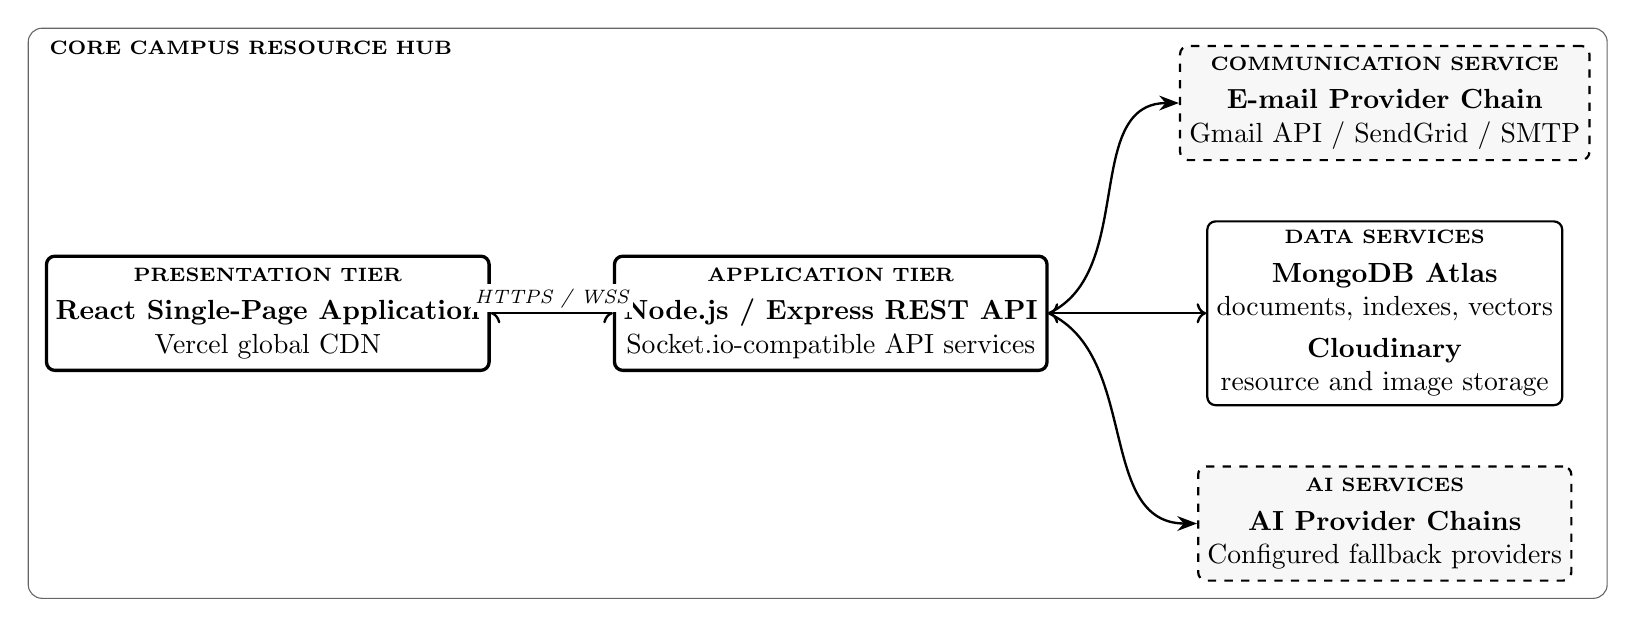
\begin{tikzpicture}[
  node distance=1.15cm and 1.25cm,
  core/.style={draw=black,line width=0.8pt,rounded corners=3pt,
               align=center,font=\normalsize,minimum height=1.45cm,
               minimum width=4.5cm,fill=white},
  primary/.style={core,line width=1.2pt,minimum width=4.8cm},
  external/.style={core,dashed,fill=black!3},
  lbl/.style={font=\scriptsize\itshape,fill=white,inner sep=1.5pt},
  arr/.style={-{Stealth[length=2.5mm]},line width=0.85pt,draw=black}]

  \node[primary] (react) {\scriptsize\bfseries PRESENTATION TIER\\[2pt]
    \textbf{React Single-Page Application}\\Vercel global CDN};

  \node[primary,right=1.55cm of react] (api)
       {\scriptsize\bfseries APPLICATION TIER\\[2pt]
        \textbf{Node.js / Express REST API}\\Socket.io-compatible API services};

  \node[core,right=2.0cm of api] (data)
       {\scriptsize\bfseries DATA SERVICES\\[2pt]
        \textbf{MongoDB Atlas}\\documents, indexes, vectors\\[3pt]
        \textbf{Cloudinary}\\resource and image storage};
  \node[external,above=0.75cm of data] (mail)
       {\scriptsize\bfseries COMMUNICATION SERVICE\\[2pt]
        \textbf{E-mail Provider Chain}\\Gmail API / SendGrid / SMTP};
  \node[external,below=0.75cm of data] (ai)
       {\scriptsize\bfseries AI SERVICES\\[2pt]
        \textbf{AI Provider Chains}\\Configured fallback providers};

  \draw[arr,<->] (react) -- node[lbl,above]{HTTPS / WSS} (api);
  \draw[arr,<->] (api.east) -- (data.west);
  \draw[arr] (api.east) to[out=25,in=180] (mail.west);
  \draw[arr] (api.east) to[out=-25,in=180] (ai.west);

  \node[draw=black!60,rounded corners=5pt,inner sep=6pt,
        fit=(react)(api)(data)(mail)(ai)] (platform) {};
  \node[font=\scriptsize\bfseries,fill=white,inner sep=2pt,
        below right=1mm and 2mm of platform.north west]
        {CORE CAMPUS RESOURCE HUB};
\end{tikzpicture}
}
\captionsetup{width=0.84\textwidth}
\caption{Three-tier system architecture, data services, and external integrations}
\label{fig:arch}
\end{figure}

\subsection{System Workflow}
Figure~\ref{fig:workflow} shows the complete system workflow. After
OTP-verified signup and JWT login, users reach a role-aware
dashboard from which all eleven functional flows branch out:
resources, events, clubs, lost-and-found, announcements, chat,
notifications, AI search, admin panel, and profile management. The
central design pattern shared by moderated content flows is
\emph{create $\rightarrow$ safety scan $\rightarrow$ auto-publish
when fully clean, otherwise human review $\rightarrow$ notify}.

\reportwidefig{workflow-diagram.pdf}{User access, resource moderation,
publication, campus services, and notification workflow}{fig:workflow}

\subsection{User Roles}
Access control follows a three-tier role model. Table~\ref{tab:roles}
summarizes what each role is allowed to do; every privileged API
route enforces these rules through the \texttt{authorize} middleware.
\begin{table}[htbp]
\centering
\caption{User roles and their permissions}
\label{tab:roles}
\begin{tabular}{@{}p{2.4cm}p{11cm}@{}}
\toprule
\textbf{Role} & \textbf{Permissions} \\
\midrule
Student & Browse/search all published content; upload resources;
          post lost-and-found items; RSVP to events; join clubs;
          chat; download resources; manage own profile. \\
Moderator & All student permissions, plus: review resources and
          lost-and-found posts; inspect AI-flagged items; create and
          manage events, clubs, and announcements;
          block/unblock users. \\
Admin & All moderator permissions, plus: change user roles; delete
          users; full platform statistics. \\
\bottomrule
\end{tabular}
\end{table}

\section{Database Design}
The database consists of twelve MongoDB collections. Their fields
and relationships are shown in the entity--relationship diagram
(Figure~\ref{fig:erd}) and summarized in
Table~\ref{tab:collections}. The \texttt{User} collection is the
hub: nearly every other collection references it. Moderation fields are stored on the resource and lost-and-found models, while staff-created modules apply their own validation and publication rules.

\reportwidefig{erd-diagram.pdf}{MongoDB collections for authorization,
academic content, communication, and AI-assisted retrieval}{fig:erd}

\begin{table}[htbp]
\centering
\caption{Summary of database collections}
\label{tab:collections}
\begin{tabular}{@{}lp{9.6cm}@{}}
\toprule
\textbf{Collection} & \textbf{Purpose and key fields} \\
\midrule
User & Account data: name, unique e-mail and student ID,
  department, role, bcrypt-hashed password, block status. \\
AuthOtp & Hashed signup / password-reset OTPs with TTL index for
  automatic expiry. \\
Resource & Study material metadata: course, department, semester,
  file info, Cloudinary IDs, moderation verdict, downloads, rating. \\
Announcement & Notice content, priority, scheduled
  \texttt{publishAt}, expiry, read receipts, attachments. \\
Event & Date/time/location, capacity (0 = unlimited), RSVP
  registrations (going / maybe / declined), club reference. \\
Club & Name, category, join policy (open / request), members with
  roles (member / officer), pending join requests. \\
LostFoundItem & Item type (lost / found), private contact info,
  claim list with statuses, resolution timestamps. \\
Conversation & Direct or group chat thread: members, admins, last
  message reference. \\
Message & Sender, text, attachments, reply reference, delivered-to
  and seen-by lists. \\
Notification & Per-user feed entries with type, link, and read
  flag. \\
Embedding & 384-dimensional vector, source type + ID (polymorphic),
  content hash to skip unnecessary re-embedding. \\
ResourceChunk & Ordered text or safe-image-description passage,
  parent resource, passage type, and 384-dimensional embedding. \\
\bottomrule
\end{tabular}
\end{table}

\section{API Design}
The REST API is organized into nine route groups, protected by two
middleware layers: \texttt{protect} (JWT verification) and
\texttt{authorize} (role check).

\begin{table}[htbp]
\centering
\caption{REST API route groups (representative endpoints)}
\label{tab:api}
\begin{tabular}{@{}llp{6.6cm}@{}}
\toprule
\textbf{Group} & \textbf{Base path} & \textbf{Representative operations} \\
\midrule
Auth & \texttt{/api/auth} & signup, verify-signup-otp, login,
  forgot/reset password, profile update \\
Resources & \texttt{/api/resources} & upload, list/filter, preview,
  file stream, download count \\
Announcements & \texttt{/api/announcements} & create, approve, pin,
  mark read, attachment stream \\
Events & \texttt{/api/events} & create, approve, register, RSVP
  update, cancel \\
Clubs & \texttt{/api/clubs} & create, join/leave, decide request,
  set member role \\
Lost-Found & \texttt{/api/lost-found} & post, claim, decide claim,
  resolve, reopen \\
Chat & \texttt{/api/chat} & conversations, messages, group
  management, AI assistant (stream) \\
Notifications & \texttt{/api/notifications} & list, mark read,
  clear \\
Admin & \texttt{/api/admin} & statistics, user list, role change,
  block, delete \\
\bottomrule
\end{tabular}
\end{table}

\section{Security Design}
Security measures are applied at every layer:
\begin{itemize}[itemsep=2pt]
  \item \textbf{Account security}: e-mail ownership proven by OTP
        before account creation; OTPs stored only as hashes with
        automatic TTL expiry and attempt counting; passwords hashed
        with bcrypt (salt rounds = 10).
  \item \textbf{Transport / headers}: HTTPS everywhere, Helmet
        security headers, strict CORS allow-list.
  \item \textbf{Abuse prevention}: express-rate-limit (3{,}000
        requests per 15 minutes per IP); upload size and type
        validation with Multer.
  \item \textbf{Authorization}: JWT verification middleware plus
        role checks on every privileged route; chat access verified
        per conversation membership.
  \item \textbf{Content safety}: automated screening on resources and other safety-sensitive publishing flows; flagged or partially inspected items remain unpublished for human review.
  \item \textbf{Privacy}: lost-and-found contact details hidden by
        default and revealed only to approved claimants; passwords
        excluded from all API responses.
\end{itemize}

% ------------------------------------------------------------

\chapter{Methodology}
\label{ch:method}

\section{Implementation Workflow}
The system was implemented as a sequence of independently verifiable modules. Data models and protected API routes were completed before their corresponding user interfaces, followed by real-time functions, content processing, semantic indexing, and administrative controls. Automated tests and role-based manual checks were repeated after integration.


% ------------------------------------------------------------
After a successful login, every user lands on a role-aware dashboard
(Figure~\ref{fig:dashboard}) that summarizes platform activity ---
total resources, announcements, upcoming events, and open
lost-and-found items --- and provides quick access to recent
resources and the latest announcements. The persistent left
navigation and the top ``Ask AI'' search bar are available from
every page.

\reportfig{dashboard.png}{Role-aware dashboard with activity summary
cards, recent resources, and latest announcements}{fig:dashboard}

\section{Authentication and OTP Verification}
Signup collects name, e-mail, student ID, department, and password.
The server generates a six-digit OTP, stores its hash in the
\texttt{AuthOtp} collection with a TTL expiry, and e-mails it via
the configured e-mail provider chain. Only after correct OTP entry is the account created with
the default \texttt{student} role. Login returns a signed JWT; a
parallel OTP flow handles forgotten passwords.

\reportfig{auth-login.png}{Login and signup with e-mail OTP
verification}{fig:auth}

\section{Resource Upload and AI Moderation Pipeline}
Users can author in-application text or blog resources and upload PDF, DOCX, PPTX, XLSX, image, TXT, or ZIP attachments with course, department, and semester metadata. The file goes to Cloudinary;
text and images are then extracted server-side (pdf-parse, Mammoth,
canvas) and scanned through a provider chain: Groq first, Hugging
Face second, and OpenAI last. Clean, fully inspected uploads are
published automatically. Flagged files, partial extractions, and
provider-unavailable checks fail safely into the moderator review
queue; they are never auto-published. Rejection notifies the uploader
with a reason. Searchable passages are generated asynchronously for
approved text and safe image descriptions.

\reportfig{resource-upload.png}{Resource upload with metadata and
moderation status}{fig:upload}
\reportfig{resource-browse.png}{Browsing, filtering, previewing and downloading published resources}{fig:browse}

\section{Events with Capacity-Aware RSVP}
Moderators create events with date, time, location, and optional
capacity. Students RSVP as \emph{going}, \emph{maybe}, or
\emph{declined}; registration is blocked once capacity is reached.
Users see their events in a calendar view, and posters or admins can
cancel events, which notifies registrants.

\reportfig{events.png}{Event listing and RSVP flow}{fig:events}

\section{Clubs with Join Policies and Member Roles}
Each club declares a join policy: \emph{open} (instant membership)
or \emph{request} (application with an optional note, decided by an
officer or the creator). Members hold \emph{member} or
\emph{officer} roles; officers manage requests and membership.

\reportfig{clubs.png}{Club directory and membership
management}{fig:clubs}

\section{Lost and Found with Claim Workflow}
Users post lost or found items with photos. Contact information is
hidden by default. Another user files a claim with a note; the
poster (or a moderator) approves or rejects it. Approval reveals
contact details to the claimant only and moves the item to
\emph{claimed}, then \emph{resolved}. This protects personal data
while still reuniting items with owners.

\reportfig{lostfound.png}{Lost-and-found listing and claim
dialog}{fig:lostfound}

\section{Announcements with Scheduled Publishing}
Announcements carry a priority (normal / important / urgent),
optional attachments, a scheduled \texttt{publishAt} time, and an
optional expiry. The scheduled publication time controls visibility; persistent background notification scheduling remains deployment-dependent.
Read receipts record which students have seen each notice.

\reportfig{announcements.png}{Announcement feed with priority
badges}{fig:announcements}

\section{Real-Time Chat}
Chat supports direct and group conversations over Socket.io.
Messages support attachments, replies, and editing; the system
tracks per-user seen status. Group admins can rename
groups, add or remove members, and promote other admins. All chat
REST endpoints re-verify conversation membership server-side.

\reportfig{chat.png}{Real-time direct and group messaging with seen
receipts}{fig:chat}

\section{Notifications}
Every significant action --- new message, approved or rejected
upload, event change, claim decision, announcement --- creates a
notification document and pushes it live over Socket.io. The bell
menu supports mark-as-read, mark-all, and clear.

\section{Semantic Search and AI Assistant}
When content is published, its title and body are embedded with a
multilingual MiniLM sentence-transformer running inside the Node
process (Transformers.js); the 384-dimensional unit vector is stored
in the \texttt{Embedding} collection, one shared collection for all
five content types. A content hash prevents redundant re-embedding
when text has not changed. Queries embed the user's question and run
Atlas \texttt{\$vectorSearch}; results are re-checked against each
source collection's visibility rules, so search can never leak
unpublished content. The AI assistant wraps this pipeline and
streams its answer token-by-token over server-sent events. The
assistant is reachable from the ``Ask AI about resources'' bar at the
top of every page (visible in Figure~\ref{fig:dashboard}).

For resource files, extracted text and safe image descriptions are
split into overlapping ordered chunks and embedded separately in the
\texttt{ResourceChunk} collection. Retrieval first applies the
current user's resource-visibility filter, then ranks matching
passages and metadata together. The assistant can therefore answer
questions about what a PDF contains, summarize a DOCX file, or
describe an indexed image while citing numbered, clickable source
cards. Exact-title and lexical-passage matches outrank weaker legacy
semantic matches.

\section{Admin Panel}
The panel shows platform statistics (users, resources, pending
approvals), a user-management table (block/unblock, delete, role
change --- role change restricted to admins), and review queues for pending resources and lost-and-found items, together with management tables for staff-created content.

\reportfig{admin.png}{Admin panel: statistics and review tools}{fig:admin}

\section{Deployment}
The web frontend and the current backend entry points are configured for Vercel deployment. The live web application is available at \href{https://campus-resource-hub-frontend.vercel.app/}{Campus Resource Hub}. MongoDB Atlas stores application documents, embeddings, and vector-search indexes, while Cloudinary stores resource files and images. Environment variables isolate provider credentials and deployment-specific settings. The companion React Native application currently presents the deployed web application inside a WebView with back-navigation and retry handling; a fully native API client remains future work.

% ------------------------------------------------------------

\chapter{Results and Analysis}
\label{ch:results}
% ------------------------------------------------------------
\section{Achieved Features}
All objectives set in Chapter 1 were implemented and verified
manually across the three roles:

\begin{table}[htbp]
\centering
\caption{Feature completion summary}
\label{tab:results}
\begin{tabular}{@{}p{5.2cm}p{8.2cm}@{}}
\toprule
\textbf{Feature} & \textbf{Status / observed behaviour} \\
\midrule
OTP signup \& JWT login & Accounts created only after correct OTP;
  expired OTPs auto-deleted by TTL index. \\
Resource sharing & Upload, preview, download, and view counting work for supported file resources; in-application text resources are also supported. \\
AI moderation & Harmful, partially inspected, or provider-unavailable
  resource uploads are quarantined; clean fully inspected files may auto-publish. \\
Review workflow & Available for resources and lost-and-found;
  rejection reasons are delivered as notifications, while staff-created
  events and announcements follow their own validation rules. \\
Events & Capacity limit enforced at registration time; RSVP status
  editable; calendar view correct. \\
Clubs & Open clubs join instantly; request clubs require officer
  decision; roles enforced. \\
Lost \& found & Contact hidden until claim approval; item lifecycle
  open $\rightarrow$ claimed $\rightarrow$ resolved. \\
Chat & Real-time delivery with seen receipts; group
  administration functions. \\
Semantic search & Meaning-based matches returned with sources; AI
  assistant streams answers. \\
Admin panel & Statistics, user management and resource and lost-and-found review queues operational. \\
\bottomrule
\end{tabular}
\end{table}

\section{Security Analysis}
The two-layer moderation pipeline proved effective in testing:
AI-flagged uploads never became publicly visible, while clean and
fully inspected uploads were auto-published. Partial extraction or
provider failure sent content to human review instead of failing
open. Rate limiting blocked request floods with HTTP 429 responses.
JWT tampering attempts were
rejected by signature verification, and role-guarded endpoints
returned HTTP 403 for insufficient roles. Lost-and-found contact
details were confirmed to be absent from API responses until a claim
was approved.

\section{Bug Report and Resolution Log}
The Git history of both repositories was reviewed to distinguish
implemented fixes from planned work. Table~\ref{tab:buglog} records
the principal defects that affected safety, search correctness,
real-time connectivity, or usability. Commit hashes provide
traceable implementation evidence; merged pull requests represent
the authoritative state on the \texttt{main} branches.

\begin{longtable}{@{}>{\raggedright\arraybackslash}p{1.15cm}
  >{\raggedright\arraybackslash}p{4.15cm}
  >{\raggedright\arraybackslash}p{5.15cm}
  >{\raggedright\arraybackslash}p{3.1cm}@{}}
\caption{Resolved defect log derived from Git history and regression tests}
\label{tab:buglog}\\
\toprule
\textbf{ID} & \textbf{Observed defect and impact} &
\textbf{Root cause and implemented resolution} &
\textbf{Evidence / status} \\
\midrule
\endfirsthead
\toprule
\textbf{ID} & \textbf{Observed defect and impact} &
\textbf{Root cause and implemented resolution} &
\textbf{Evidence / status} \\
\midrule
\endhead
BR-01 & Graphic, adult, or otherwise unsafe files could be approved
when a vision provider failed or only part of a document was
extracted. This was the highest-severity publication risk. &
The earlier path treated incomplete inspection too optimistically.
Moderation now fails safe: flagged, partial, and provider-unavailable
results remain unpublished for human review. Deterministic text
screening and the Groq--Hugging Face--OpenAI provider order were also
added. & \texttt{df5fa96}; four moderation-policy regression tests
pass. Resolved. \\
\addlinespace
BR-02 & The AI assistant could find a resource by title but could not
reliably explain what was inside its PDF or Office document. &
Only short metadata and a limited excerpt were searchable. The first
repair stored file excerpts (\texttt{d356801}); the completed repair
adds ordered overlapping \texttt{ResourceChunk} passages, embeddings,
safe image descriptions, and an existing-resource backfill. &
\texttt{d356801}, \texttt{0e707b3}; 54 approved resources indexed
with zero extraction failures. Resolved. \\
\addlinespace
BR-03 & Content questions could rank weakly related legacy semantic
matches above an exact title or file-passage match, producing noisy
sources. &
Metadata and passage relevance had comparable scores. The final
hybrid rank gives exact titles and lexical file passages stronger
weight, loads ordered passages for summary intent, and preserves
inline source numbering. & \texttt{0e707b3}; real PDF-summary and
deadlock-query checks place the relevant Operating Systems resources
first. Resolved. \\
\addlinespace
BR-04 & A semantic/vector result risked bypassing the visibility rules
used by ordinary keyword queries. &
Vector candidates were not sufficient authorization evidence. Every
candidate is now joined back through the same approved/owner/role
filter before its passages are exposed. & \texttt{c755663},
\texttt{0e707b3}; streaming test returned zero unauthorized sources.
Resolved. \\
\addlinespace
BR-05 & Real-time chat connections were unreliable after frontend
deployment on Vercel. &
The Socket.io client transport did not match the deployed network
path. The client now prefers explicit WebSocket transport with
deployment-compatible connection settings. & \texttt{42ef620}; fix
merged to frontend \texttt{main}. Resolved. \\
\addlinespace
BR-06 & Expanding the header AI input to multiple lines changed the
header height and obscured adjacent controls; an interim revert also
removed desired behavior. &
The textarea participated in normal header layout. It now grows in an
absolutely positioned layer, retains Enter/Shift+Enter behavior, and
shows readable Markdown plus numbered source cards. &
\texttt{757141d}, \texttt{f4259f7}, \texttt{16edb5f},
\texttt{641b1bc}; production build passes. Resolved. \\
\bottomrule
\end{longtable}

\subsection{Current Verification Snapshot}
The current repository suites were executed after the latest pull. The backend completed 27 of 27 tests, the frontend completed 6 of 6 tests, and the mobile wrapper completed 1 of 1 test. These suites cover security-sensitive moderation behavior, search authorization, client behavior, and mobile rendering at the unit or integration level. They do not replace a controlled production load test, but they provide repeatable evidence that the checked application paths pass in the current source state.

\subsection{Open Operational Constraint}
Third-party artificial-intelligence services impose quotas and can become temporarily unavailable. The application handles this condition conservatively: content that cannot be inspected completely is not auto-published, and configured fallbacks are attempted where appropriate. Provider availability and credit usage must therefore be monitored independently from functional application defects.

\section{Verification and Capacity Limitations}
No controlled concurrency or endurance benchmark is stored in the repositories, so earlier capacity figures are not presented as measured results. Table~\ref{tab:test-summary} reports the reproducible automated verification that is available. Before campus-wide deployment, the system should be tested with representative file uploads, semantic searches, simultaneous Socket.IO connections, and third-party provider failures under monitored production-like conditions.

\begin{table}[htbp]
\centering
\caption{Automated test-suite results for the current repositories}
\label{tab:test-summary}
\begin{tabular}{L{4cm}ccc}
\toprule
\textbf{Application} & \textbf{Passed} & \textbf{Failed} & \textbf{Result} \\
\midrule
Backend API and services & 27 & 0 & \textbf{Pass} \\
Frontend application & 6 & 0 & \textbf{Pass} \\
Mobile wrapper & 1 & 0 & \textbf{Pass} \\
\bottomrule
\end{tabular}
\end{table}

\section{Cost and Deployment Considerations}
The development deployment uses managed services including Vercel, MongoDB Atlas, Cloudinary, and external e-mail and artificial-intelligence providers. Free service tiers can support development and demonstration, but their quotas, cold starts, execution limits, and provider availability are operational constraints rather than guaranteed capacity. Production adoption therefore requires measured load testing, quota monitoring, a background-job strategy for content processing, and a documented service budget.

\chapter*{Conclusion and Future Work}
\addcontentsline{toc}{chapter}{Conclusion and Future Work}
% ------------------------------------------------------------
This project set out to replace the fragmented, unmoderated channels
through which campus information currently flows with a single,
secure, intelligent platform. The delivered system --- Campus
Resource Hub --- implements verified onboarding, a categorized study-resource repository, capacity-aware events, club
management, a privacy-preserving lost-and-found process, scheduled
announcements, real-time messaging with seen state, and a semantic AI assistant, supported by targeted content-safety workflows and role-based
access control. The implementation demonstrates that modern
techniques usually associated with large commercial platforms ---
AI content moderation, vector-based semantic search, streamed LLM
assistance --- can be integrated into a student project integrated with managed cloud services. All current automated suites passed, while production-scale concurrency remains to be established through controlled load testing. Beyond its immediate utility,
the project provided deep practical experience in full-stack
architecture, real-time systems, applied AI services, and cloud
deployment.

\section*{Future Work}
% ------------------------------------------------------------
Planned improvements include:
\begin{enumerate}[itemsep=2pt]
  \item \textbf{Fully native mobile client} --- replace the implemented React Native WebView shell with dedicated native screens that consume the existing REST and real-time interfaces.
  \item \textbf{Background job queue} --- moving AI scanning and
        embedding generation off the request path (e.g.\ BullMQ) to
        remove the largest CPU spike.
  \item \textbf{Push notifications} --- Web Push / FCM so users are
        reachable when the site is closed.
  \item \textbf{Richer analytics} --- per-department dashboards,
        trending resources, and event attendance reports.
  \item \textbf{Federated login} --- university e-mail SSO (OAuth2)
        alongside OTP signup.
  \item \textbf{Horizontal scaling} --- multiple backend instances
        with a Socket.io Redis adapter once campus-wide load
        requires it.
  \item \textbf{Accessibility and localization} --- full Bangla
        interface and WCAG-compliant UI review.
\end{enumerate}

% ------------------------------------------------------------

% ===========================================================================
% REFERENCES
% ===========================================================================
\begingroup
\small
\bibliographystyle{ieeetr}
\bibliography{references}
\endgroup

% ===========================================================================
% APPENDIX
% ===========================================================================
\appendix
\chapter{Supplementary Material}

\section{Code Availability}
The live application and complete project source are available at the following addresses:
\begin{itemize}[leftmargin=*,itemsep=6pt]
  \item \textbf{Live web application}\\[-2pt]
        {\small\url{https://campus-resource-hub-frontend.vercel.app/}}
  \item \textbf{Web frontend repository}\\[-2pt]
        {\small\url{https://github.com/KaziAkibRayhan/campus-resource-hub-frontend}}
  \item \textbf{Backend API repository}\\[-2pt]
        {\small\url{https://github.com/KaziAkibRayhan/campus-resource-hub-backend}}
  \item \textbf{Mobile wrapper repository}\\[-2pt]
        {\small\url{https://github.com/KaziAkibRayhan/campus-resource-hub-mobile}}
\end{itemize}

\begin{center}
{\color{black}\qrcode*[height=27mm]{https://campus-resource-hub-frontend.vercel.app/}}\\[4pt]
{\small Scan to open the live web application.}
\end{center}

\section{Current Automated Verification}
At the time of final formatting, the checked repository state completed 27 backend tests, 6 frontend tests, and 1 mobile test without failures. Production-scale load testing and formal user-acceptance testing remain outside the scope of these automated suites.

\end{document}
